%!TEX root = ../doc.tex
\documentclass[../doc.tex]{subfiles}

\begin{document}
\chapter{Introduction}
\Gls{trt} is a dominant mechanism of energy transfer in the high energy density regimes found in astrophysical phenomena and \gls{icf} experiments. In these regimes, the thermal radiation emitted by all matter at a temperature greater than zero is emitted in the ``soft X-ray'' range corresponding to a wavelength of $\sim\!\SI{1}{\nano\meter}$. By contrast, the human body emits radiation in the infrared regime corresponding to $\sim\!\SI{10}{\micro\meter}$. 
Furthermore, these high energy density regimes are often extreme enough that matter emits and absorbs radiation enough that its motion is altered. 
That is, the radiation field is strong enough to impact the pressure and momentum matter experiences. This tightly coupled interplay between the motion of matter and thermal radiative heat transfer is characterized by the field of radiation-hydrodynamics. Here, we focus on the ``radiation'' part of radiation-hydrodynamics. 

Kinetic models of photon transport phenomena are regarded as first-principles models for \gls{trt}. These models are believed to be a key component in reducing the gap between simulation and experiment observed in \gls{hedp} experiments. 
Kinetic models are capable of capturing the physics that cheaper models (e.g.~radiation diffusion) miss but at the cost of orders of magnitude more computational work and memory usage. 
In fact, the kinetic TRT package used in radiation-hydrodynamics simulations of the \gls{nif} often occupies 90\% of the runtime and memory usage of the entire simulation. Algorithms that reduce the cost of modeling TRT can thus have a significant impact on the cost of the entire simulation, allowing scientists to perform faster design iterations and realize higher accuracy models for the same electricity bill. 
Existing codes are extremely optimized so reductions in time-to-solution must come from the development of novel algorithms. 

In this dissertation, numerical algorithms for efficiently solving the kinetic description of radiation's interaction with matter are developed, the aim being to design methods that can be readily extended and incorporated into the radiation-hydrodynamics codes used to model \gls{nif}. The algorithms are centered around the use of the radiation moment equations to accelerate the iterative solution of the kinetic equation. The kinetic equation is used to define closures for the moment system so that, upon convergence, the moment system can reproduce the physics of the kinetic equation. 
Iterative acceleration is achieved through a bidirectional coupling: the kinetic equation informs the moment system through closures while the moment system drives the kinetic equation by computing the slow-to-converge physics. Such algorithms are attractive in the context of radiation-hydrodynamics since the moment system can be directly coupled to the hydrodynamics equations providing separation between the expensive kinetic equation and the evolution of stiff multiphysics. 

The primary challenge in the development of these algorithms is the efficient numerical approximation of the moment system. The closures used to define the moment system can make the application of existing discretization techniques and efficient preconditioned iterative solvers difficult. In addition, we target high-order discretizations techniques in order to align with the methods in use for hydrodynamics simulations of \gls{nif}. The development of high-order discretizations for the moment system that can be efficiently solved with existing linear solver technology is the primary contribution presented in this dissertation. 

In this chapter, we \todo{introduce}

\section{Motivation}
\subsection{The National Ignition Facility}
\gls{nif} is laser-based \gls{icf} research facility located at the \gls{llnl}. At the time of writing this dissertation, NIF houses the world's largest and most energetic laser consisting of 192 beamlines. The target bay of \gls{nif} is shown in Fig.~\ref{intro:nif} inside which the 192 beamlines converge onto the interior surface of the dime-sized, cylindrical halhraum (depicted in Fig.~\ref{intro:halhraum}) at the center of target chamber. The walls of the halhraum heat to extreme temperatures, creating an X-ray oven that bathes a BB-sized capsule of frozen hydrogen isotopes at the center of the halhraum. The X-rays burn the fuel initiating an ablation that compresses the fuel to densities and pressures comparable to those seen at the center of the sun allowing the hydrogen isotopes to fuse into helium and release tremendous energy. In August 2021, NIF was able to achieve a burning plasma where the fusion reaction was sustained by energy released by the fusion process \cite{Zylstra2022}. This achievement represents a 10x improvement over previous attempts and is an important step toward achieving ignition, where the the fusion reaction is maintained entirely by energy released from fusion. 
% --- NIF pictures --- 
\begin{figure}
\centering
\begin{subfigure}{.49\textwidth}
	\centering
	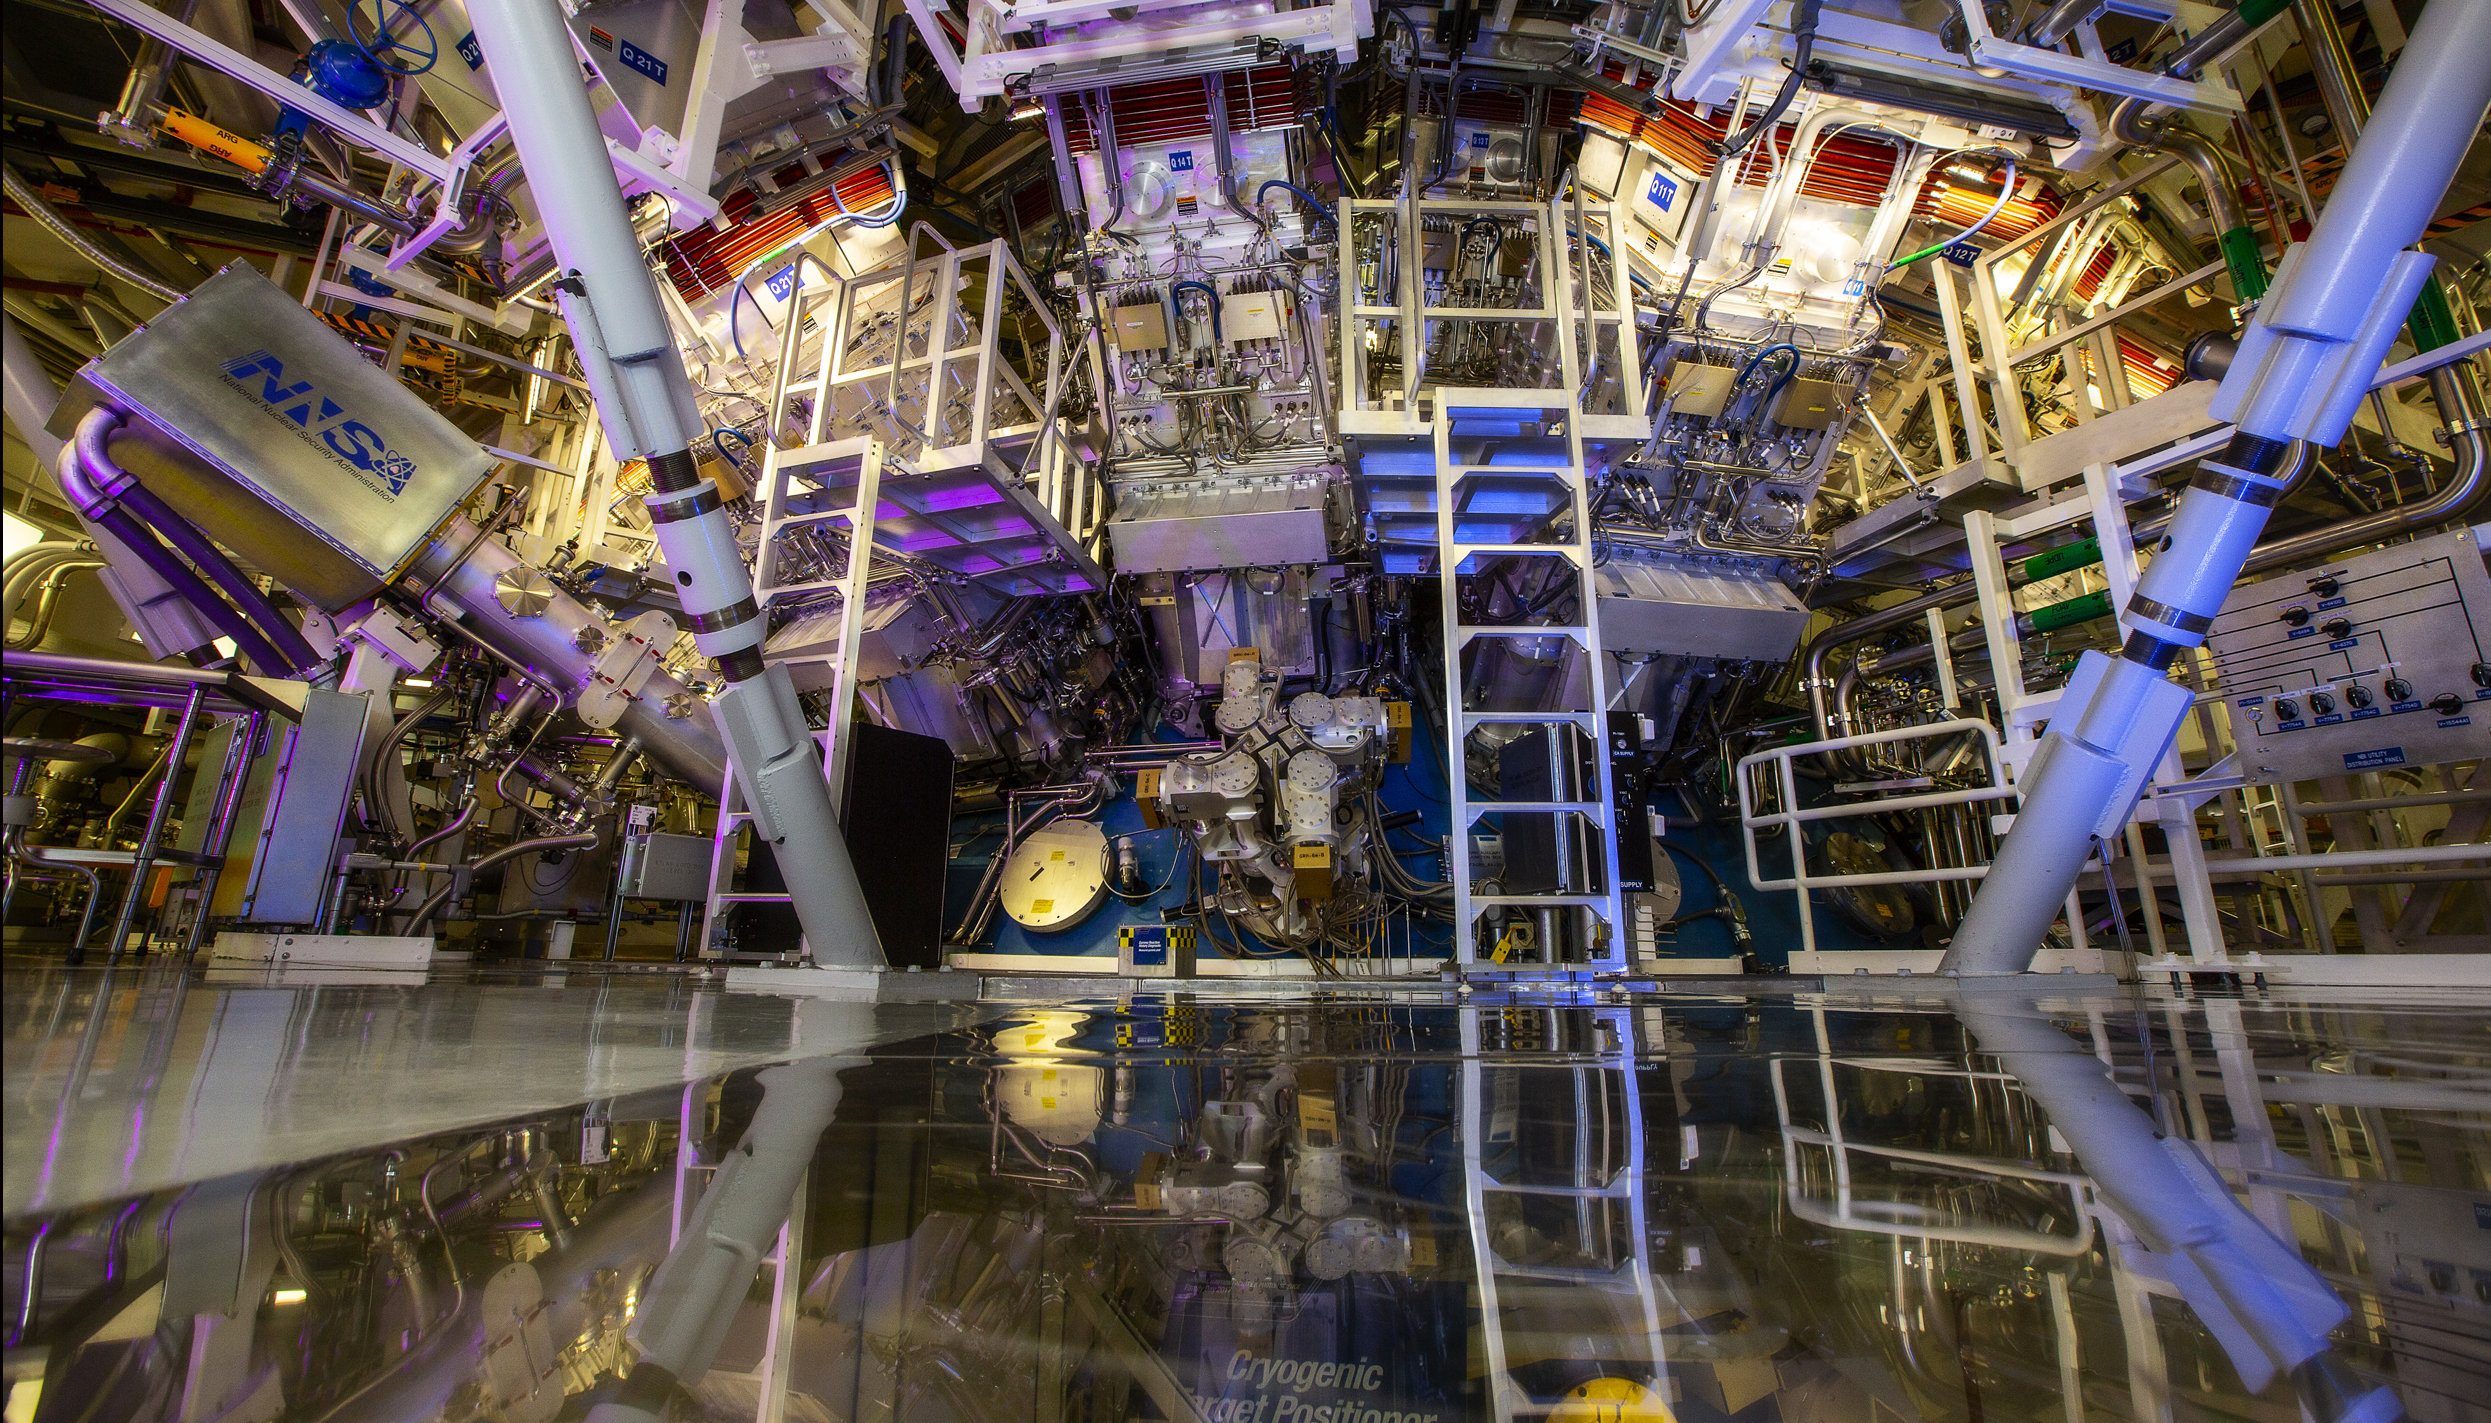
\includegraphics[height=1.75in]{data/img/nif.jpg}
	\caption{}
	\label{intro:nif}
\end{subfigure}
\begin{subfigure}{.49\textwidth}
	\centering
	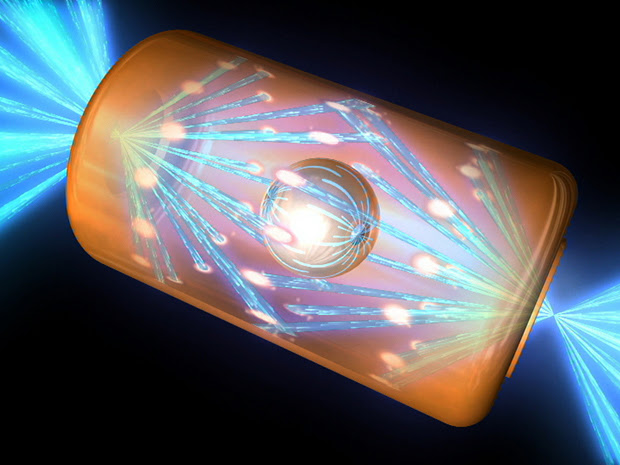
\includegraphics[height=1.75in]{data/img/halhraum.jpeg}
	\caption{}
	\label{intro:halhraum}
\end{subfigure}
\caption{(a) a photograph of the National Ignition Facility's target bay showing the laser entrance ports and diagnostics for measuring the properties of the experiment. (b) a depiction of the halhraum placed in the center of the target chamber shown in (a). The lasers impinge on the interior surface of the halhraum by entering through two openings on each side of the cylindrical halhraum. The walls of the halhraum heat to extreme temperatures, releasing X-rays that bathe the hydrogen fuel at the center of the halhraum. }
\end{figure}

The primary physical processes involved in a NIF experiment are: \gls{trt}, plasma physics, and nuclear reactions. Thermal radiation emitted by the walls of the halhraum is the primary driver of the ablation that initiates the fusion reaction. The extreme temperatures and pressures present inside the halhraum mean matter exists in an ionized, plasma state where electrons are stripped free leaving a positively charged nucleus. This separation of charges induces electric and magnetic fields which greatly expand the range of possible motions and significantly complicate the study of their behavior. Finally, nuclear reactions are responsible for the production of fusion energy and the release of reaction byproducts, such as neutrons, that are an invaluable component for measuring the yield of a NIF experiment. 
The numerical simulation of these physical processes, along with many others, comprise a simulation suite that allows scientists to design better experiments and gain insight into the physics of \gls{icf} without the need for expensive and time-consuming physical experimentation. 

\subsection{Thermal Radiative Transfer}
The focus of this dissertation is the development of numerical models for simulating the release and deposition of thermal energy. 

\subsection{Curved Meshes and High-Order Finite Elements}
Recent trends in computer architecture, namely the ending of Moore's Law\footnote{the empirical observation that the number of transistors in an integrated circuit doubles every two years.}, indicate computers will be increasingly parallel and dependent on domain specific architectures such as \glspl{gpu}. This is especially evident in the Top500 list\footnote{a ranked list of the world's 500 most powerful supercomputers.}: from June 2010 to June 2020, the average number of CPU cores per socket rose from 4 to 20. In that same time span, the number of GPU-accelerated supercomputers increased from none to 134 \todo{(citation needed, dates likely wrong)}. Furthermore, it has been observed that floating point throughput is improving faster than memory latency and bandwidth. Thus, data movement will become increasingly expensive relative to computation. For GPU-accelerated computers, data movement is further compounded by the need to transfer data to and from the GPU. 

In light of these trends, the Department of Energy's Center for Efficient Exascale Discretizations (CEED) within the Exascale Computing Project (ECP) has targeted high-order finite element methods as one of it's main research thrusts. Compared to low-order methods, high-order methods are more accurate for the same number of unknowns (on smooth problems) and have better data reuse and locality. In other words, high-order methods have a higher floating point to memory access ratio\footnote{this ratio is called the \emph{arithmetic intensity}.} that makes them more amenable to efficient implementation on emerging \gls{hpc} architectures. 

In particular, the next-generation radiation-hydrodynamics code for modeling \gls{nif} at \gls{llnl} is based around the use of high-order finite elements on high-order (curved) meshes. In hydrodynamics simulations, high-order methods that use curved meshes have been shown to provide greater robustness (especially in the presence of significant mesh distortions), symmetry preservation, and strong scaling when compared to low-order methods \cite{blast,blast2,blast3}. In this framework, the material's velocities are represented with continuous finite elements and the thermodynamics variables are represented with discontinuous finite elements. This approach ensures the interfaces in the mesh remain continuous while allowing thermodynamic conservation to hold locally on each element. 
Figure \ref{intro:3p_anim} shows the evolution of the mesh associated with a third-order Lagrangian hydrodynamics simulation referred to as the ``triple point problem.'' In Lagrangian simulations, the mesh moves with the materials in order to preserve material interfaces exactly. Thus, as the materials deform, so does the mesh, leading to the deformed curved interfaces seen in the final mesh of Fig.~\ref{intro:3p_anim}. 
% --- triple point problem --- 
\begin{figure}
\centering
\foreach \f in {0,40,120,156}{
	\begin{subfigure}{.49\textwidth}
		\centering
		\includegraphics[width=\textwidth]{data/img/3p_anim/triple-\f.png}
		\caption{}
	\end{subfigure}
}
\caption{Selected time steps of the triple point problem. A third-order finite element representation is used to describe the mesh. A Lagrangian hydrodynamics approach is used where the mesh deforms with the materials in order to preserve material interfaces. This leads to the severely distorted curved elements depicted at the final time step. It is on such a mesh that we would like to solve radiation transport on. }
\label{intro:3p_anim}
\end{figure}

Coupling TRT to high-order hydrodynamics requires a transport method that is in some sense compatible with curved meshes. One possibility is to leverage existing transport methods by approximating the high-order mesh by refining it and using straight-edged elements. This approach, referred to as the low-order refined approach, is depicted for an example quadratic quadrilateral element in Fig.~\ref{intro:lor}. Note that is approach necessarily increases the number of unknowns, depicted as the nodes in each element, in the problem. 
\textcite{graph_sweeps} showed that realistic meshes generated from a high-order Lagrangian hydrodynamics code required a significant number of refinements to avoid simulation failure arising from inverted elements. In the context of the already memory and computation intensive 7-dimensional transport problem, this option can be impractical.   
In addition, the low-order refined approach under severe mesh distortions may not always produce an admissible mesh. 
Figure \ref{intro:lor_dist} shows an example of a distorted third-order element where the low-order refined process leads to an ill-defined mesh containing inverted and overlapping elements in addition to elements with poor aspect ratios. In such case, a method that solves on the high-order mesh could continue whereas a low-order refined method would cause the simulation to fail. 
% --- low order refined simple --- 
\begin{figure}
\centering
\foreach \f in {lor.pdf,lor_1.pdf,lor4_1.pdf}{
	\begin{subfigure}{.32\textwidth}
		\centering
		\includegraphics[width=\textwidth]{figs/\f}
		\caption{}
	\end{subfigure}	
}
\caption{Depictions of the low-order refined process. (a) shows a quadratic quadrilateral element that has four unkowns. (b) and (c) show linear approximations to the geometry of the element in (a) that use one and two refinements, respectively. In order for the curved surfaces to be accurately captured refinements are required. However, this necessarily increases the number of unknowns which can be impractical in the context of the already memory intensive radiation transport solve. }
\label{intro:lor}
\end{figure}
% --- low order refined impractical --- 
\begin{figure}
\centering
\foreach \f in {lor_dist.pdf,lor_dist_1.pdf,lor_dist4_1.pdf}{
	\begin{subfigure}{.32\textwidth}
		\centering
		\includegraphics[width=\textwidth]{figs/\f}
		\caption{}
	\end{subfigure}	
}
\caption{Depictions of the low-order refined process on a very distorted, cubic element. In this case, refining the high-order geometry shown in (a) leads to elements with poor aspect ratios, inverted elements, and elements that overlap. This is an example where naively refining the element would lead to simulation failure and is a motivating example for the need to solve on the high-order mesh.}
\label{intro:lor_dist}
\end{figure}

Radiation transport methods compatible with curved meshes are desired in order to avoid the necessary increase in unknowns and reduced robustness associated with the low-order refined approach. It is also possible that high-order methods could be beneficial in terms of accuracy and multiphysics compatibility with high-order hydrodynamics. However, these claims of increased accuracy and compatibility have yet to be demonstrated in large-scale tightly coupled simulations. Discontinuous finite element representations of the energy density (scalar flux in nuclear engineering terminology) are preferred in order to have immediate multiphysics compatibility with the framework of \cite{blast}. High-order discontinuous finite element methods for radiation transport have received attention recently with the development of \gls{dg} discretizations of the \gls{sn} transport equations compatible with curved meshes in \cite{graph_sweeps,woods_thesis} and corresponding \gls{dsa} methods in \cite{ldrd_dsa,doi:10.1080/00295639.2020.1799603}. However, high-order discretizations of the VEF equations compatible with curved meshes have not yet been developed. 

\section{The Variable Eddington Factor Method}
% VEF, its applications, and broad benefits 
The \gls{vef} method \cite{mihalas}, also known as \gls{qd} \cite{goldin}, is a rapidly-converging nonlinear scheme for solving the Boltzmann transport equation. VEF has been applied to a wide range of transport and multiphysics problems including (but not limited to) nuclear reactor eigenvalue problems \cite{airstova_eigenvalue}, nuclear reactor kinetics \cite{doi:10.13182/NSE13-42}, and \gls{trt} \cite{anistratov1996nonlinear}. It performs well in problems having both optically thick and thin regions and treats anisotropic scattering equally well \cite{anistratov_fvm,ARISTOVA2000139}. Robust convergence is achieved by iteratively coupling the transport equation to the VEF equations, a moment-based equivalent reformulation of transport. The exact closures used to form the VEF equations are weak functions of the solution meaning even simple iterative schemes, such as fixed-point iteration, converge rapidly. 

VEF offers significant algorithmic flexibility in that any valid discretization of the VEF equations will yield a rapidly-converging algorithm. This is in stark contrast to \gls{dsa} which places severe restrictions on the discretization of the moment equations in order to guarantee stability \cite{A}. In the case where the VEF and transport discretizations are not algebraically consistent, referred to as a VEF method with an ``independent'' discretization \cite{doi:10.1080/00411459308203810,two-level-independent-warsa}, the discrete solutions of the transport and VEF equations will differ on the order of the discretization error and will be equivalent only in the limit as the mesh is refined. However, even in an under-resolved problem, VEF still produces a ``transport solution'' in that the solution of the VEF method is a discrete solution of an equivalent reformulation of the transport equation. Furthermore, VEF methods generally preserve the thick diffusion limit \cite{diflim} and have conservation even if the transport discretization in isolation does not. These properties are particularly useful in multiphysics calculations since the lower-dimensional VEF equations can be directly coupled to the other physics components in place of the high-dimensional transport equation. In addition, discretizations for the transport and VEF equations can be designed independently so that they are in some sense optimal for their intended uses. 

% examples of benefits 
This flexibility has been exploited to improve efficiency in relation to all seven dimensions of the transport equation. 
% time 
\textcite{GHASSEMI2020109315} showed that different order temporal discretizations can be applied to the transport and VEF equations. Ongoing work suggests that time-stepping stability and accuracy can be maintained when just one transport inversion is performed per time step \cite{yee_mc21}. \textcite{anistratov2021implicit} used data compression techniques to reduce storage costs in time-dependent calculations. In astrophysics, VEF is used to simplify the implementation of coupling TRT to hydrodynamics and to avoid the memory cost of solving the time-dependent transport equation \cite{Jiang_2012,GNEDIN2001437,GEHMEYR1994320}. 
% space 
\textcite{Davis_2012} used a short characteristics discretization of the transport equation. \textcite{me} and \textcite{LOU2019258} designed a spatial discretization of the VEF equations to increase multiphysics compatibility. This algorithm was used to form the basis of an efficient radiation-hydrodynamics method in \cite{LOU2021110393}. \textcite{YEE2020109696} showed that robust convergence is maintained even when positivity-preserving methods are used inside the iteration. 
% energy
\textcite{ANISTRATOV2019186} solved the multigroup TRT equations by using a VEF method with multiple levels in frequency. It is also well-known that the multigroup eigenvalue problem can be solved with only the need for eigenvalue iterations on the one-group VEF equations \cite{AL}. 

The above techniques rely on the efficient solution of the discretized VEF equations. VEF methods reduce the overall cost of the simulation by trading inversions of the high-dimensional transport equation with inversions of the lower-dimensional VEF equations. In all of VEF's applications, the solution of the discretized VEF equations is buried under multiple nested loops corresponding to time integration, Newton iterations, eigenvalue iterations, multi-group iterations, and/or fixed-point iterations. The efficient iterative solution of the VEF equations is then crucial to the efficiency of the overall algorithm and is a prerequisite for the practicality of any VEF method. 

The unusual structure of the VEF equations and their lack of self-adjointness make the development of discretizations and their corresponding preconditioned iterative solvers difficult.
While considerable effort has been placed into the discretization of the VEF equations, to our knowledge, existing methods either rely on expensive and unscalable preconditioners such as block incomplete LU (BILU) factorization, cannot be solved with interation counts independent of the mesh size, or do not mention solvers entirely. Previous work on discretizing the VEF equations includes finite volume \cite{anistratov_fvm,doi:10.1080/00411459308203810,QDBC,Jiang_2012,Jones2019TheQM}, finite difference \cite{WIESELQUIST2014343}, mixed finite element \cite{vallette,me,olivier_mandc,LOU2019258}, continuous finite element \cite{wieselquist,two-level-independent-warsa}, and discontinuous finite element \cite{dima_dfem} techniques. Most VEF methods are designed to be algebraically consistent with their application's discretized transport equation which typically requires discretizing the first-order form of the VEF equations. Such discretizations solve for both the zeroth and first moment of the solution and thus have significantly more unknowns than discretizations of the second-order form. In addition, block preconditioners \cite{benzi_golub_liesen_2005} are required to efficiently solve discretizations of the first-order form. Such solvers can require nested iteration for robustness (see \cite{warsa_mfem} for a radiation diffusion example). 

\textcite{two-level-independent-warsa} showed that VEF methods with and without algebraic consistency converge equivalently as long as the transport data is properly represented. In particular, computing the Eddington tensor and boundary factor using finite element interpolation and \gls{sn} angular quadrature enables rapid convergence for any valid discretization of the VEF equations. An independent discretization of the second-order form of the VEF equations then has the potential to provide the rapid convergence of a consistent VEF method while solving for fewer unknowns and avoiding the need for block preconditioners. Such a method also has the flexibility to discretize the VEF equations in a manner that can leverage existing linear solver technology.

\section{Research Scope and Objectives}

\section{Outline}

\end{document}